\chapter[Appendix]{Appendix}
\label{Appendix}
\section{Thesis website}
The ongoing developments of this thesis research and a gallery of moving Semantic Form models are available on the following website: 

\url{https://studiomto.square.site/thesis-what-may-be-known-2024}

\section{LaTeX manuscript repository}
The following web page provides access to the LaTeX code used to compile this thesis, including all figures and formatting details:

\url{https://github.com/orusmateo/Orus-MCS-Thesis}

\section{Moving and interactive models}
The following web page provides access to the moving and interactive models developed for my thesis. 

\url{https://studiomto.square.site/moving-semforms}

\section{Semantic Forms surface and volume equations }
\label{Semantic Forms equations}
\begin{table}[h]
    \centering
    \begin{tabular}{|l|l|l|}
\hline
 & \textit{Volume (V)} & \textit{Surface (S)} \\[10pt]
 \hline
cone &  $\pi r^2 \frac{h}{3}$ & $\pi r \sqrt{r^2+h^2}$  \\[10pt] \hline
 cylinder & $\pi r^2 h$ & $2 \pi r h$ \\[10pt]
  \hline
sphere & $\frac{4}{3} \pi  R^3$ & $4 \pi r^2$ \\[10pt] \hline
horn torus & $2 \pi^2 a^3$ & $4 \pi^2 a^2$ \\[10pt] \hline
ring torus & $\frac{1}{4} \pi^2(R+r)(R-r) a^*$ & $\pi^2 (R+r)(R-r)$ \\[10pt]
\hline
\multicolumn{3}{l}

    \end{tabular}
    %\caption{Caption}
\end{table}

\begin{quote}
    \centering *Pappus’s centroid theorem \citep{weisstein_torus_nodate}.
\end{quote}

\index[people]{Pappus}
\clearpage

\section{Application of Sarajlić et al. configurations to three-dimensional graphlets}
As part of my style guide for Query Isomorphs analysis I propose that the Sarajlić et al. graphlet configurations \citep[p. 3]{sarajlic_graphlet-based_2016} can be used for graph input and graph analysis.

\begin{figure}[h!]
    \centering
    \includegraphics[width=0.8\textwidth]{figures/5.6.png}
    \caption[Example Query Isomorph in two dimensions and three dimensions assembled from directed graphlets]{\textbf{Example Query Isomorph in two dimensions and three dimensions assembled from directed graphlets.} \\
(a) From Sarajlić et al. 2016’s point b, “Illustration of how directed graphlets assemble together to form complex networks”, from “Figure 1. Illustration of directed graphlets” \citep[p. 3]{sarajlic_graphlet-based_2016}. In keeping with Sarajlić et al., the whole network can be created by adding graphlet G4, G1, and G3, meaning that in the process a new graphlet, G2, was created. The colours red, green, blue, and black are sourced from \citep[p. 3]{sarajlic_graphlet-based_2016}. (b) Spatial arrangement adds semantic value of verticality to communicate hierarchy of the blue node.  Red nodes are querying for nodes in both higher and lateral hierarchy. (c) Other arrangements can easily facilitate different relationships in the Query Isomorph. (b) and (c) The colours red, green, blue, are sourced from \citep[p. 3]{sarajlic_graphlet-based_2016} here also, but white is used instead of black for contrast. Black nodes in this example are all placed in a lateral level of hierarchy. In a functional Query Isomorph platform, nodes could also be placed higher or lower to each other. Furthermore, the angles and directions of these graphlets are presented for simplicity of the variety they can have, but does not represent the diversity of angle and form that graphlets can be configured in as Query Isomorphs. 
}
    \label{f5.6}
\end{figure}
\clearpage


\section{The Semantic Forms located in Bertin’s taxonomy of network graphs}
\begin{figure}[h!]
    \centering
    \includegraphics[width=0.9\textwidth]{figures/A.3.png}
    \caption[Groups of imposition and types of imposition]{\textbf{Groups of imposition and types of imposition} \citep[p. 52]{bertin_semiology_2011}.
From \textit{Semiology of Graphics: Diagrams, Networks, Maps} by Jacques Bertin, translated by William J. Berg. Reprinted by permission of the University of Wisconsin Press. © 1983 by the Board of Regents of the University of Wisconsin System. All rights reserved.}
    \label{fig:A3}
\end{figure}
%\clearpage
\begin{figure}[h!]
    \centering
    \includegraphics[width=\textwidth]{figures/A.4.png}
    \caption[Groups of imposition and types of imposition as categories for my Semantic Shapes, Semantic Forms, and three-dimensional gigamaps]{\textbf{Groups of imposition and types of imposition as categories for my Semantic Shapes, Semantic Forms, and three-dimensional gigamaps}. My work is overlaid onto Bertin’s categorization of network diagrams \citep[p. 52]{bertin_semiology_2011} from \textit{Semiology of Graphics: Diagrams, Networks, Maps} by Jacques Bertin, translated by William J. Berg. Reprinted by permission of the University of Wisconsin Press. © 1983 by the Board of Regents of the University of Wisconsin System. All rights reserved.}
    \label{fig:A4}
\end{figure}
%\clearpage
\begin{figure}[h!]
    \centering
    \includegraphics[height=0.8\textheight]{figures/A.5.png}
    \caption[Implantation and imposition of network diagrams]{\textbf{Implantation and imposition of network diagrams} \citep[p. 270]{bertin_semiology_2011} \\
From \textit{Semiology of Graphics: Diagrams, Networks, Maps} by Jacques Bertin, translated by William J. Berg. Reprinted by permission of the University of Wisconsin Press. © 1983 by the Board of Regents of the University of Wisconsin System. All rights reserved.}
    \label{fig:A5}
\end{figure}
\begin{figure}[h!]
    \centering
    \includegraphics[width=\textwidth]{figures/A.6.png}
    \caption[Implantation and imposition of network diagrams as categories for my Semantic Shapes, Semantic Forms, and three-dimensional gigamaps]{\textbf{Implantation and imposition of network diagrams as categories for my Semantic Shapes, Semantic Forms, and three-dimensional gigamaps.} \citep[p. 270]{bertin_semiology_2011} 
My work is overlaid onto Bertin’s categorization of network diagrams \citep[p. 270]{bertin_semiology_2011} from \textit{Semiology of Graphics: Diagrams, Networks, Maps} by Jacques Bertin, translated by William J. Berg. Reprinted by permission of the University of Wisconsin Press. © 1983 by the Board of Regents of the University of Wisconsin System. All rights reserved.
}
    \label{fig:A6}
\end{figure}
\clearpage


\section{Graphical abstract}
\begin{figure}[h!]
    \centering
    \includegraphics[width=\textwidth]{figures/AF1.pdf}
    \caption[Graphical abstract]{\textbf{Graphical abstract}}
    \label{fig:graphical_abstract}
 \clearpage
\end{figure}
\clearpage


\section{Horn of futures}
\FloatBarrier
\begin{figure}[h!]
    \centering
    \includegraphics[width=\textwidth]{figures/5.29.png}
    \caption[Horn of Futures]{\textbf{Horn of Futures.} This figure depicts the 2D dimensional reduction of the bottom view of a modified 3D Cone of Plausibility \citep[p. 14]{taylor_creating_1990} \citep[p. 73]{bezold_overview_1993}. This Cone Semantic Form is curved into a spiral similar to \autoref{fig:18} “Diagram of a design process with iterations” \citep[p. 343]{sevaldson_designing_2022} \citep{sevaldson_designing_2022-1}. The 3D version of this form twists like a ram’s horn, and this thesis involves the study of the horn torus, hence the name \textit{Horn of Futures}}
    \label{f5.29}
\end{figure}
\FloatBarrier
\clearpage







\section{Horn Torus point cloud}
\begin{figure}[h!]
    \centering
        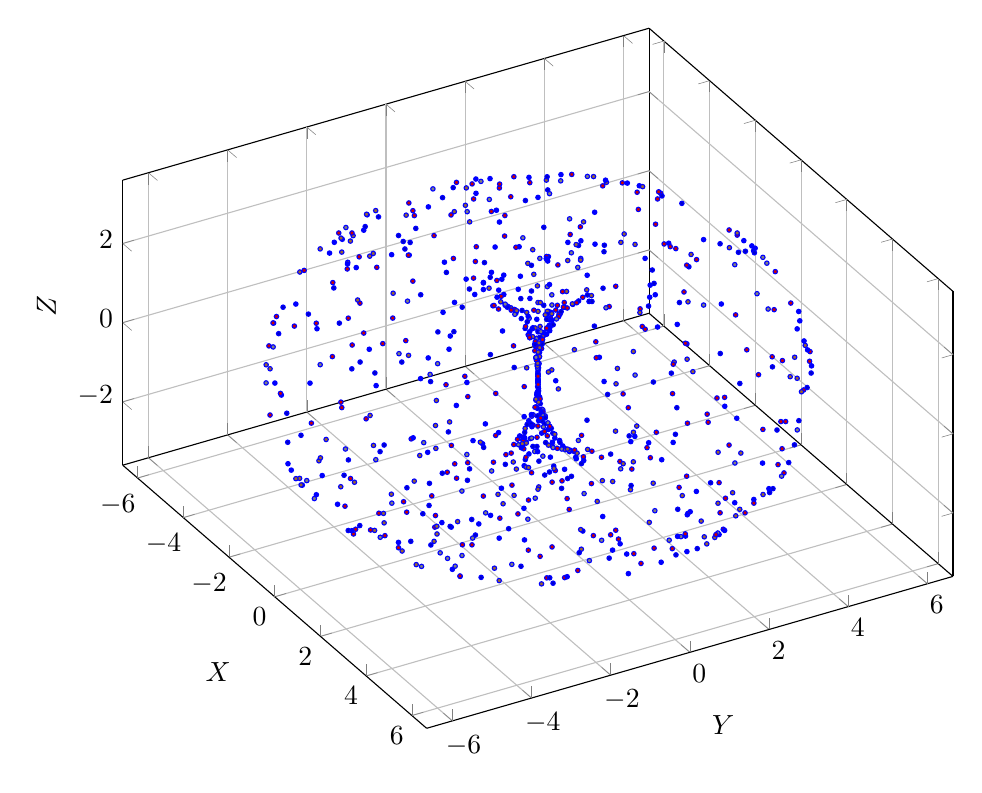
\begin{tikzpicture}
          \begin{axis}[
                view={60}{30},
                width=\textwidth, 
                axis equal,
                grid=major,
                xlabel={$X$},
                ylabel={$Y$},
                zlabel={$Z$},
        %        title={Random Points Inside a Horn Torus},
                samples=50,
                domain=0:360,
                y domain=0:360
            ]
            
            % Define parameters for a horn torus
            \pgfmathsetmacro{\R}{3}  % Major radius, set equal to minor radius
            \pgfmathsetmacro{\r}{3}  % Minor radius, set equal to major radius
            \pgfmathsetmacro{\thickness}{0.7} % Thickness to control the spread within the torus tube
        
            % Generate random points inside the horn torus
            \foreach \i in {1,...,888} {
                \pgfmathsetmacro{\theta}{random(0, 360)}
                \pgfmathsetmacro{\phi}{random(0, 360)}
                \pgfmathsetmacro{\radialDist}{\r + random(-\thickness, \thickness)}
                \pgfmathsetmacro{\x}{(\R + \radialDist * cos(\phi)) * cos(\theta)}
                \pgfmathsetmacro{\y}{(\R + \radialDist * cos(\phi)) * sin(\theta)}
                \pgfmathsetmacro{\z}{\radialDist * sin(\phi)}
        
                \addplot3+[only marks, mark=*, mark size=0.8pt, color=blue] coordinates {(\x, \y, \z)};
            }
            \end{axis}
        \end{tikzpicture}
    \caption[Horn Torus point cloud]{\textbf{Horn Torus point cloud.} Created for LaTeX with the help of ChatGPT 4o.}
    \label{Wolfram Horn Torus}
\end{figure}
\clearpage



\section{The Data Visualisation Catalogue by Severino Ribecca}

\begin{figure}[h!]
    \centering
    \includegraphics[height=0.8\textheight]{figures/A.2.png}
    \caption[The Data Visualisation Catalogue]{\textbf{The Data Visualisation Catalogue.} 
\citep{ribecca_data_2017}. Used with permission.}
    \label{fig:A.2}
\end{figure}

\clearpage

\section{Semantic Field \textit{S}}

\begin{multicols}{4}
\begin{enumerate}[label=\arabic*.]
\item A Dish with One Spoon
\item abduction
\item Abundant Intelligences project
\item academic cross-pollination
\item academic knowledge management (AKM)
\item accessibility
\item Artificial General Intelligence (AGI)
\item AI energy consumption
\item algorithm
\item analogy
\item anti-oppression
\item Artificial Intelligence (AI)
\item axiological paradigms
\item biocultural memory
\item biodynamic agriculture
\item Blender
\item blind spots
\item Boundary Critique
\item capitalist extractivist economy
\item ChatGPT
\item Circle Semantic Shape
\item classification of natural forms
\item climate crisis
\item climate crisis mitigation
\item climate hyperobject
\item climate resilience
\item Carbon dioxide (CO2)
\item collaborative co-creation
\item collaborative Knowledge Production
\item colligative theory formation
\item complexity management
\item composition
\item Computational Analysis of Texts and Graphs (CATG)
\item computational graphesis
\item computational semiosis
\item conceptual gateways
\item Conceptual Graphs
\item Conceptual Networks
\item Cone Semantic Form
\item Cones of Plausibility
\item consilience
\item consilience across disciplines
\item Consilience in Knowledge Activation (CKA)
\item Consilience of Inductions
\item consolation
\item constellationary fields
\item conversational model
\item Creation-as-Research
\item Creative Presentations of Research
\item criminal justice system
\item Critical Systems Thinking (CST)
\item cybernetic mycelium
\item cybernetic rhizome
\item Cylinder Semantic Form
\item data activation
\item data hierarchy
\item data hierarchy visualization
\item data ontology modeling
\item data-information-knowledge-wisdom hierarchy (DIKW)
\item data-to-knowledge transformation
\item database of databases
\item decentralized knowledge structure
\item decomposition
\item deduction
\item degree-difference
\item Design for Health (DH)
\item Design for Sustainability Transitions (DfST)
\item Design with a Capital D
\item desolation
\item diagrammatic reasoning
\item Digital Humanities
\item dimensional addition
\item dimensionality
\item disciplinary interchange
\item discourse fields
\item domain models
\item double cone in optics
\item Double-Cone Semantic Form
\item double-diamond shape
\item eco-justice
\item ecoanthroposymbiosis
\item ecojustice
\item ecological cost of AI
\item ecologically informed AI strategy
\item Embedding Projector
\item energy resources
\item Entity-Relationship (ER) diagrams
\item environmental crisis
\item environmental degradation
\item environmental sustainability
\item epistemological diversity
\item Epistemology
\item Equity-Centered Community Design
\item Equity-Centered Community Design (ECCD)
\item ethnobotany
\item ethnoecology
\item Euclidean
\item evidence synthesis
\item filtration
\item formation and growth in morphology
\item funnel plot
\item futures cone
\item general consilience (GC)
\item Generous AI
\item geometric compositions
\item Gestalt psychology
\item gigamapping
\item glass box AI
\item Global Assortativity
\item Global Topological Synchronization (GTS)
\item GPT-3
\item GPT-4
\item graph embeddings
\item graph isomorphology
\item graph LLMs
\item graph morphology
\item graph of concepts
\item graph-based ontology models
\item graphesis
\item graphical user interface (GUI)
\item graphically structured knowledge
\item graphlet interface
\item graphlets
\item hierophanic
\item HITL (Human-in-the-Loop)
\item HITL CATG KA
\item Horn of Futures
\item Horn Torus Semantic Form
\item Human Analysis of Text and Graphs (HATG)
\item humanistic interface design
\item hyper-specialization
\item hyperlinked bibliometric graphing
\item hyperobject
\item incipit
\item Inclusive Design (ID)
\item induction
\item information design
\item information overload
\item information visualization
\item information visuospatialization
\item InfraNodus
\item interbeing
\item interdisciplinarity
\item interdisciplinary consilience
\item interdisciplinary Knowledge co-Production
\item interdisciplinary Knowledge Production
\item interdisciplinary synthesis
\item interdisciplinary topic mapping
\item Intergovernmental Panel on Climate Change (IPCC)
\item interpretable AI
\item isomorphic interbeing
\item isomorphogenesis
\item isomorphology
\item knowledge abstraction and synthesis
\item Knowledge Activation (KA)
\item knowledge design studio laboratory
\item knowledge engineering
\item knowledge graphs
\item Knowledge Management (KM)
\item Knowledge Production (KP)
\item Knowledge Production for Sustainability Transitions (KPST)
\item Knowledge Production through composition
\item Knowledge Production through visuospatial Knowledge Form composition
\item Knowledge Pyramid
\item Knowledge Surfacing (KS)
\item Knowledge Surfacing, Synthesis, Translation, and Creation(KSSTP)
\item Knowledge Synthesis (KS)
\item Knowledge Translation (KT)
\item knowledge work platforms
\item KP quantification
\item Large Language Model (LLM)
\item logoi
\item logos of form
\item Logseq
\item Loop-line
\item Low-dimensional topology
\item ludic quality
\item major diameter
\item major radius
\item manual node placement
\item Markdown language
\item material infrastructure
\item Meru Chakra
\item meta-analysis
\item meta-language
\item meta-Systematic Combining (MSC)
\item metaphysics
\item methodological framework
\item methodological pluralism
\item middle ontology
\item minor diameter
\item minor radius
\item Mistral 7B
\item MNIST handwritten digits database
\item monocrops
\item morphology
\item moving spatial network graphs
\item multi-dimensional network graphs
\item multi-mathematical approach
\item multi-scale topological data features
\item natural resources
\item network graph
\item network graph composition
\item network graphlet
\item network subgraphs
\item networked data visualization
\item node grouping
\item Obsidian
\item Ontological Semantic Network Summaries (OSNS)
\item ontology
\item opaque AI
\item oppressive terminology
\item Oslo School of Systemic Design
\item outer diameter
\item outer radius
\item particle accelerator of ideas
\item Perceptual Artifacts Lab (PAL)
\item permaculture
\item Persistence Homology (PH)
\item Personal Knowledge Management (PKM)
\item perspective in art
\item plant-human co-evolution
\item point cloud
\item point plot heatmap
\item power relations
\item qualitative methods
\item query graphs
\item Query Isomorphs
\item rectangular coordinate system
\item Research-Creation
\item Research-for-Creation
\item Research-from-Creation
\item researcher grouping
\item rewilding
\item Ring Torus Semantic Form
\item Roam Research
\item Semantic Field S
\item Semantic Forms
\item semantic network mapping
\item Semantic Shapes
\item Semantic Topological Semiotics
\item simplicial complex
\item Small Language Models
\item social inequality
\item social justice
\item Social Sciences and Humanities Research Council
\item spatial and temporal modeling
\item spatial composition
\item spatial network graphs
\item spatial semiotic representation
\item spatial topic model network graphs
\item Sphere Semantic Form
\item Sri Yantra
\item stakeholder
\item Sustainability Transitions Knowledge Activation (STKA)
\item studio laboratory of knowledge design
\item surfaces of revolution
\item sustainability solutions frameworks
\item Sustainability Transitions (ST)
\item symbol composition
\item Symbol-setting
\item symbolic representation
\item syntopical consilience
\item Syntopical Consilience Abduction (SCA)
\item syntopical reading
\item Syntopicon
\item Systematic Combining (SC)
\item Systemic Design
\item Systemic Design Association (SDA)
\item Systems Oriented Design (SOD)
\item Systems Theory
\item Systems Thinking
\item Topological Capta Analysis (TCA)
\item TCA Researcher Grouping
\item TCA Workspace
\item tensors
\item Terroir of Text and Graphs (TTG)
\item text graphs
\item thought forms
\item thought signs
\item three-dimensional forms
\item three-dimensional information visualization
\item three-dimensional topic models
\item topic model network graphs
\item Topic Models
\item Topological Data Analysis (TDA)
\item Topological Capta Analysis (TCA)
\item topological semiotics
\item Topology
\item toroidal manifold
\item torus
\item transdisciplinary KA (Knowledge Activation)
\item Tree of Porphyry
\item UN Sustainable Development Goals (SDGs)
\item University
\item upper ontology
\item vector embeddings
\item vector search
\item Vedic visuospatial culture
\item visual argument
\item visual epistemology
\item visual reasoning
\item visuospatial epistemology
\item visuospatial forms of knowledge production
\item visuospatial knowledge activation interface
\item visuospatial reasoning
\item weighting
\item wicked problem
\item Zettelkasten
\item Zone of Semantic Stasis
\end{enumerate}
\end{multicols}
\clearpage

\section{Adler’s 102 \textit{Great Ideas}}
The following terms are listed alphabetically as per The \textit{Great Ideas: a Syntopicon of Great Books of the Western World} (1952), derived from the texts in \textit{Great Books of the Western World} (1952).
\begin{multicols}{4} % Use 2 or 3 columns, whichever fits well
\begin{enumerate}[label=\arabic*.]
    \item Angel
    \item Animal
    \item Aristocracy
    \item Art
    \item Astronomy and Cosmology
    \item Beauty
    \item Being
    \item Cause
    \item Chance
    \item Change
    \item Citizen
    \item Constitution
    \item Courage
    \item Custom and Convention
    \item Definition
    \item Democracy
    \item Desire
    \item Dialectic
    \item Duty
    \item Education
    \item Element
    \item Emotion
    \item Eternity
    \item Evolution
    \item Experience
    \item Family
    \item Fate
    \item Form
    \item God
    \item Good and Evil
    \item Government
    \item Habit
    \item Happiness
    \item History
    \item Honor
    \item Hypothesis
    \item Idea
    \item Immortality
    \item Induction
    \item Infinity
    \item Judgement
    \item Justice
    \item Knowledge
    \item Labor
    \item Language
    \item Law
    \item Liberty
    \item Life and Death
    \item Logic
    \item Love
    \item Man
    \item Mathematics
    \item Matter
    \item Mechanics
    \item Medicine
    \item Memory and Imagination
    \item Metaphysics
    \item Mind
    \item Monarch
    \item Nature
    \item Necessity and Contingency
    \item Oligarchy
    \item One and Many
    \item Opinion
    \item Opposition
    \item Philosophy
    \item Physics
    \item Pleasure and Pain
    \item Poetry
    \item Principle
    \item Progress
    \item Prophecy
    \item Prudence
    \item Punishment
    \item Quality
    \item Quantity
    \item Reasoning
    \item Relation
    \item Religion
    \item Revolution
    \item Rhetoric
    \item Same and Other
    \item Science
    \item Sense
    \item Sign and Symbol
    \item Sin
    \item Slavery
    \item Soul
    \item Space
    \item State
    \item Temperance
    \item Theology
    \item Time
    \item Truth
    \item Tyranny and Despotism
    \item Universal and Particular
    \item Virtue and Vice
    \item War and Peace
    \item Wealth
    \item Will
    \item Wisdom
    \item World
\end{enumerate}
\end{multicols} % Use 2 or 3 columns, whichever fits well
\clearpage


\section{Authors included in \textit{Great Books of the Western World} (1952)}
The \textit{Great Books of the Western World} (1952) includes works by the following authors:
\begin{multicols}{4}
\RaggedRight Homer\\
Aeschylus\\
Sophocles\\
Euripides\\
Aristophanes\\
Herodotus\\
Thucydides\\
Plato\\
Aristotle\\
Hippocrates\\
Galen\\
Euclid\\
Archimedes\\
Apollonius\\
Nichomachus\\
Lucretius\\
Epictetus\\
Marcus Aurelius\\
Virgil\\
Plutarch\\
Tacitus\\
Ptolemy\\
Copernicus\\
Kepler\\
Plotinus\\
Augustine\\
Thomas Aquinas\\
Dante\\
Chaucer\\
Machiavelli\\
Hobbes\\
Rabelais\\
Montaigne\\
Shakespeare\\
Gilbert\\
Galileo\\
Harvey\\
Cervantes\\
Francis Bacon\\
Descartes\\
Spinoza\\
Milton\\
Pascal\\
Newton\\
Huygens\\
Locke\\
Berkeley\\
Hume\\
Swift\\
Sterne\\
Fielding\\
Montesquieu\\
Rousseau\\
Adam Smith\\
Gibbon\\
Kant\\
J. S. Mill\\
Boswell\\
Lavoisier\\
Fourier\\
Faraday\\
Hegel\\
Goethe\\
Melville\\
Darwin\\
Marx\\
Engels\\
Tolstoy\\
Dostoyevsky\\
William James\\
Freud
\end{multicols}
\clearpage





\section{Categorizing the subjects of this thesis}
\raggedcolumns
\begin{multicols}{2}

\noindent\hangindent=1.5em \textbf{Computer Science} \\
Artificial Intelligence (AI) \\
Machine Learning \\
Natural Language Processing (NLP) \\
Computational Linguistics \\
Data Science \\
Human-Computer Interaction (HCI) \\
Information Retrieval \\
Knowledge Representation and Reasoning \\
Topological Data Analysis (TDA) \\
Graph Theory \\
\vspace{4mm}

\noindent\hangindent=1.5em \textbf{Mathematics} \\
Topology \\
Geometry \\
Computational Topology \\
Mathematical Modeling \\
\vspace{4mm}

\noindent\hangindent=1.5em \textbf{Philosophy} \\
Philosophy of Information \\
Philosophy of Language \\
Epistemology \\
Semiotics \\
Philosophy of Science \\
Ontology \\
\vspace{4mm}

\noindent\hangindent=1.5em \textbf{Cognitive Sciences} \\
Cognitive Psychology \\
Cognitive Neuroscience \\
Visual Cognition \\
Embodied Cognition \\
\vspace{4mm}

\noindent\hangindent=1.5em \textbf{Information Science} \\
Knowledge Management \\
Personal Knowledge Management (PKM) \\
Information Visualization \\
Library and Information Science \\
Ontologies \\
Digital Libraries \\
\vspace{4mm}

\noindent\hangindent=1.5em \textbf{Design} \\
Systems Oriented Design (SOD) \\
Systemic Design \\
Information Design \\
Visual Communication Design \\
Human-Centered Design \\
\vspace{4mm}

\noindent\hangindent=1.5em \textbf{Digital Humanities} \\
Computational Humanities \\
Digital Scholarship \\
Humanistic Interface Design \\
\vspace{4mm}

\noindent\hangindent=1.5em \textbf{Interdisciplinary Studies} \\
Sustainability Transitions \\
Environmental Studies \\
Climate Science \\
Ecojustice \\
Indigenous Studies \\
Decolonizing Methodologies \\
\vspace{4mm}

\noindent\hangindent=1.5em \textbf{Linguistics} \\
Computational Linguistics \\
Semantics \\
Pragmatics \\
Language and Thought \\
\vspace{4mm}

\noindent\hangindent=1.5em \textbf{Education} \\
Knowledge Activation \\
Collaborative Learning \\
\RaggedRight Interdisciplinary Education \\
Educational Technology \\
\vspace{4mm}

\noindent\hangindent=1.5em \textbf{Sociology} \\
Sociology of Knowledge \\
Science and Technology Studies (STS) \\
Cultural Studies \\
\vspace{4mm}

\noindent\hangindent=1.5em \textbf{Communication Studies} \\
Media Studies \\
Information Theory \\
Symbolic Communication \\
\vspace{4mm}

\noindent\hangindent=1.5em \textbf{Ethnography and Anthropology} \\
Ethnoecology \\
Ethnobotany \\
Cultural Anthropology \\
\vspace{4mm}

\noindent\hangindent=1.5em \textbf{Visual Studies} \\
Visual Epistemology \\
Visual Reasoning \\
Visual Semiotics \\
Graphical Representation \\
\end{multicols}

\clearpage

\section{Experts interviewed}
I acknowledge with professional admiration the subject matter experts who provided formative feedback for this thesis. I list them here alphabetically by surname:
\begin{itemize}
    \item Dr. Evan Timothy Barba of Georgetown University
    \item Tega Brain of New York University (NYU)
    \item Antionette D. Carroll, founder of the Institute of Equitable Design and Justice and Creative Reaction Labs (CRXLAB)
    \item John P. Comer of the Redress Movement
    \item Dr. Sara Diamond, OCAD University Research Chair, Director of the Visual Analytics Lab, and Co-investigator of the OCAD U Abundant Intelligences A Dish with One Spoon – Towards “Generous AI” Invention and Collaboration project.
    \item Dr. Michael Doser of the European Council for Nuclear Research/Conseil Européen pour la Recherche Nucléaire (CERN)
    \item Ekaterina Grgurić of the University of British Columbia (UBC)
    \item Michael Groenendyk of Concordia University
    \item Micki Kaufman of the City University of New York (CUNY)
    \item Dr. Peter Jones and Cheryl May of the Systemic Design Association (SDA)
    \item Amanda Licastro of Swarthmore College
    \item Dr. Gavin Mendel-Gleason of TerminusDB
    \item Dr. Lennart Nacke, Dr. Blake Madill, and Antonio Muñoz Gomez of the University of Waterloo
    \item Rahul Nayak of the Indian Institute of Technology (IIT)
    \item Dr. Paul Pangaro of the American Society for Cybernetics (ASC)
    \item Dr. Dmitry Paranyushkin of Nodus Labs
    \item Santiago Ortiz of Moebio
    \item Serkan Özkaya, conceptual artist
    \item Ryan J. A. Murphy of the University of Newfoundland
    \item Dr. Birger Sevaldson of the Oslo School of Architecture and Design (AHO)
    \item Peter Scott of the Rotman School of Management, University of Toronto and OCAD U
    \item Dr. Maria Simakova of the University of Toronto (U of T)
    \item Brian Sunter of the University of Florida (UF)
    \item Kirsta Stapelfeldt and David Kwasny of the University of Toronto (U of T) Scarborough Digital Scholarship Unit
\end{itemize}
\clearpage

\section{Research presentations}

\noindent\hangindent=1.5em  2024, \textit{Systems Oriented Disruptions}, presented for the annual International Innovation Forum hosted by the Strategic Foresight and Innovation (SFI) program in the OCAD University School of Graduate Studies (SGS)
 
\noindent\hangindent=1.5em 2024, \textit{Systems Oriented Disruptions}, presented for Creative Disruptions// re-imagining our futures the graduate thesis exhibition by the Digital Futures (DF) program in the OCAD University’s School of Graduate Studies (SGS)

\noindent\hangindent=1.5em 2024, \textit{Body of Aesthetics}, panel discussion moderated by curator Sara Dagovic and joined by artist Artemis Han, The Gallery at Mason Studio, Toronto

\noindent\hangindent=1.5em 2023, \textit{Three-dimensional plotting of information categories using P5.js}, Perceptual Artifacts Lab (PAL) in OCAD University, moderated by the PAL Director Dr. Peter Coppin  

\noindent\hangindent=1.5em 2023, \textit{Song Within a Sacrifice Zone}, presented for “Uses and Abuses of Power in Alternative Spiritualities”, the annual conference by the Program for the Evolution of Spirituality (PES) in the Harvard Divinity School (HDS)
 
\noindent\hangindent=1.5em 2023, \textit{The biopower of faith leaders who are also alternative medicine practitioners in alternative spiritual communities}, presented for “Uses and Abuses of Power in Alternative Spiritualities”, the annual conference by the Program for the Evolution of Spirituality (PES) in the Harvard Divinity School (HDS)
 
\noindent\hangindent=1.5em 2023, \textit{Knowledge Translation vs the Climate Crisis} presented for the annual colloquim hosted by the Digital Futures (DF) in the OCAD University School of Graduate Studies (SGS)
 
\noindent\hangindent=1.5em 2022, \textit{Dissonance}, presented for the Too Big To Fail Exhibition organized by the Interdisciplinary Master’s of Art, Media and Design (IAMD) in the OCAD University School of Graduate Studies (SGS)

\noindent\hangindent=1.5em 2022, \textit{Data Tori}, presented for the annual Graduate Colloquium, moderated by Duchamp scholar Dr. Julian Haladyn, in the OCAD University School of Graduate Studies (SGS)
  
\noindent\hangindent=1.5em 2022, \textit{Medicinallity of Symbol}, presented for the annual research panel organized by the Interdisciplinary Master’s of Art, Media and Design (IAMD), in the OCAD University School of Graduate Studies (SGS), moderated by Graduate Program Director Jay Irizawa

\section{Art exhibitions}
\noindent\hangindent=1.5em 2024, \textit{GradEx 109}, OCAD University

\noindent\hangindent=1.5em 2024, \textit{Creative Disruptions// re-imagining our futures}, Digital Futures graduate thesis exhibition, OCAD University, Waterfront Campus. 
 
\noindent\hangindent=1.5em 2024, \textit{Body of Aesthetics, curated by Sara Dagovic}, The Gallery at Mason Studio, Toronto

\noindent\hangindent=1.5em 2023, \textit{Digital Futures Open Show}, OCAD University, School of Graduate Studies

\noindent\hangindent=1.5em 2023, \textit{Song Within a Sacrifice Zone}, Harvard Divinity School, Swartz Hall
 
\noindent\hangindent=1.5em 2023, \textit{Resilience and Connection: artistic explorations of mental health}, L.R. Wilson Building, McMaster University 
 
\noindent\hangindent=1.5em 2023, \emph{Too Big to Fail}, Open Space Gallery, OCADU
 
\noindent\hangindent=1.5em 2022, \textit{The Incomplete}, The Great Hall Gallery, OCADU
\clearpage

\section{Resources and tools used in this thesis}
\begin{multicols}{2}

\noindent\hangindent=1.5em \textbf{LLMs} \\
Chat GPT 3 \\
Chat GPT 4 \\
Chat GPT 4o \\
Google Gemini Advanced \\
Mistral 7B Open Orca* \\
Zephyr* \\
* set up using Ollama \\
\vspace{4mm}

\noindent\hangindent=1.5em \textbf{Computational Text Graph Tools} \\
InfraNodus \\
\RaggedRight \hangindent=1.5em  InfraNodus Chrome extension for its 3D knowledge graph \\
MIT’s SIMILE Timeline widget, run on Zotero \\
Obsidian Canvas, core plugin \\ 
Obsidian Outline, core plugin \\
Obsidian Graph View, core plugin \\
\RaggedRight \hangindent=1.5em Obsidian 3D Graph v1.0.5, community plugin by Alexander Weichart \\
Python 3.8.12 \\
PiVis* \\
Pandas Dataframes* \\
NetworkX* \\
Voyant Tools \\
* Python libraries \\
\vspace{4mm}
\noindent\hangindent=1.5em \textbf{Personal Knowledge Management (PKM)} \\
Obsidian \\
Logseq \\
Logseq PDF reader \\
Readwise Official Plugin v1.4.9 \\
Roam Research \\
\vspace{4mm}
\noindent\hangindent=1.5em \textbf{Three-Dimensional Forms} \\
Blender node programming \\
\vspace{4mm}
\noindent\hangindent=1.5em \textbf{Source Management} \\
Zotero \\
\RaggedRight \hangindent=1.5em Zotero Better BibTex extension v 6.7.202 by Emiliano Heyns (to generate citation keys) \\
Zotero Connector Chrome extension \\
\vspace{4mm}
\noindent\hangindent=1.5em \textbf{Document Drafting} \\
Google Docs \\
Google Chrome extension DocsAfter Dark \\
Microsoft Word \\
\RaggedRight \hangindent=1.5em Pandoc for populating Better BibTex citation keys into in-sentence citation and list of references \\
\RaggedRight \hangindent=1.5emLaTeX for populating Better BibTex citation keys (generated in Zotero) into in-sentence citation and list of references \\
\vspace{4mm}
\noindent\hangindent=1.5em \textbf{Document Reading} \\
Readwise \\
Readwise Reader \\
\RaggedRight \hangindent=1.5em Readwise Chrome extension (synced to Logseq and Obsidian) \\
Apple Photos Optical Character Recognition \\
Adobe Acrobat \\
Adobe Digital Editions \\
\vspace{4mm}
\noindent\hangindent=1.5em \textbf{Infinite Canvas Text Analysis Tools} \\
Miro \\
Scapple \\
\vspace{4mm}
\noindent\hangindent=1.5em \textbf{Image Management} \\
Apple Photos \\
Affinity \\
Affinity Designer \\
Affinity Publisher \\
Pinterest \\
QuickTime Player \\
\vspace{4mm}
\noindent\hangindent=1.5em \textbf{Audio and Video Production} \\
\RaggedRight Final Cut Pro \\ 
\RaggedRight Logic Pro \\
\vspace{4mm}
\noindent\hangindent=1.5em \textbf{Typefaces in Figures} \\
iA Writer Quattro S \\
Helvetica Neue \\
Arial Black \\
Avenir Next Condensed \\
\vspace{4mm}
\noindent\hangindent=1.5em \textbf{Typefaces in Document} \\
Lato for text captions \\
Noto Mono for code \\
EB Garramond for all other text \\

\end{multicols}


%\chapter*{Indices}
%\addcontentsline{toc}{chapter}{Indices}
%\label{Index}



